%Finally, an addition step was included to the fibre conditioning process, with the objective of improving the photon collection efficiency of the fibres. 

As it is demonstrated in subsection \ref{subsec:CharacterizationFibres}, the quality of the interface between the core of uncladded fibres and the environment (tritiated water in the case of TRITIUM detector) affects conspicuously the photon collection efficiency. To improve the quality of the interface, a fibre cleaning process was implemented, aiming to remove particles deposited on the fibres, such as dust and grease.  Through this cleaning process, the wetting property of the fibres is improved, as illustrated in Figure \ref{fig:WettingProperty}. The contact angle between fibres and water is decreased, preventing air molecules from attaching to the fibres and producing a uniform contact between fibres and water.
\begin{figure}[h]
\centering
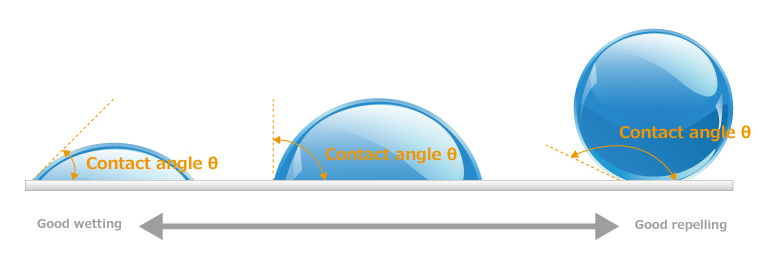
\includegraphics[scale=0.5]{4ResearchAndDevelopments/41Fibers/WettingProperty.png}
\caption{Schematic representation of the wetting properties of a flat surface (gray) in contact with a drop of liquid (blue). The wetting property is characterized by the angle formed between the surface of both objects. The smaller angle, the better wetting property of the material. \cite{WettingProperty}\label{fig:WettingProperty}}
\end{figure}
This cleaning process  was developed and carried out in the clean room of ICMOL. Three different beakers were used, the first filled with alkaline soap, the second with pure water (conductivity of the order of $10~\mu\text{S}/\cm$) and the third with isopropanol. The fibres were manually rubbed with alkaline soap during 5 minutes, afterwards introduced into the first beaker which was placed in an ultrasonic bath at $17~\kilo\hertz$ frequency during 3 minutes. Subsequently, the fibres were cleaned with a constant flow of water during 5 minutes and they were placed in the second beaker for ultrasonic bath during 3 minutes and next placed in the third beaker for ultrasonic bath during 3 minutes. Finally, the fibres were dried with a flow of gaseous $\ce{N_2}$ and kept in clean conditions until their introduction into the detector vessel. The improvement of the light collection of the scintillating fibres after this cleaning process was determined by measuring the energy spectra of a bundle of twenty uncladded fibres of $15~\cm$ length before and after undergoing this cleaning process. The setup used for this measurements is described in Figure \ref{fig:BunchWith2PMTsCoincidence}. The energy spectra were measured for the background and for a $\ce{^{90}Sr}$ and $\ce{^{137}Cs}$ radioactive sources, shown in Figures \ref{fig:ResultsOfCleaningProcessBackground} and \ref{fig:ResultsOfCleaningProcessSource}, respectively. A shift of the spectra to higher energies was observed for the clean fibres with respect to the spectra of fibres without cleaning. The equation \ref{eq:RelativeImprovement} was used to quantify the improvement achieved by the cleaning process. Although no improvement in the number of detected events was observed for the background measurement, an improvement of photon collection efficiency of a factor of $1.26$ and $1.35$ was obtained for the $\ce{^{90}Sr}$ and $\ce{^{137}Cs}$ sources, respectively.

\begin{figure}[h]
\centering
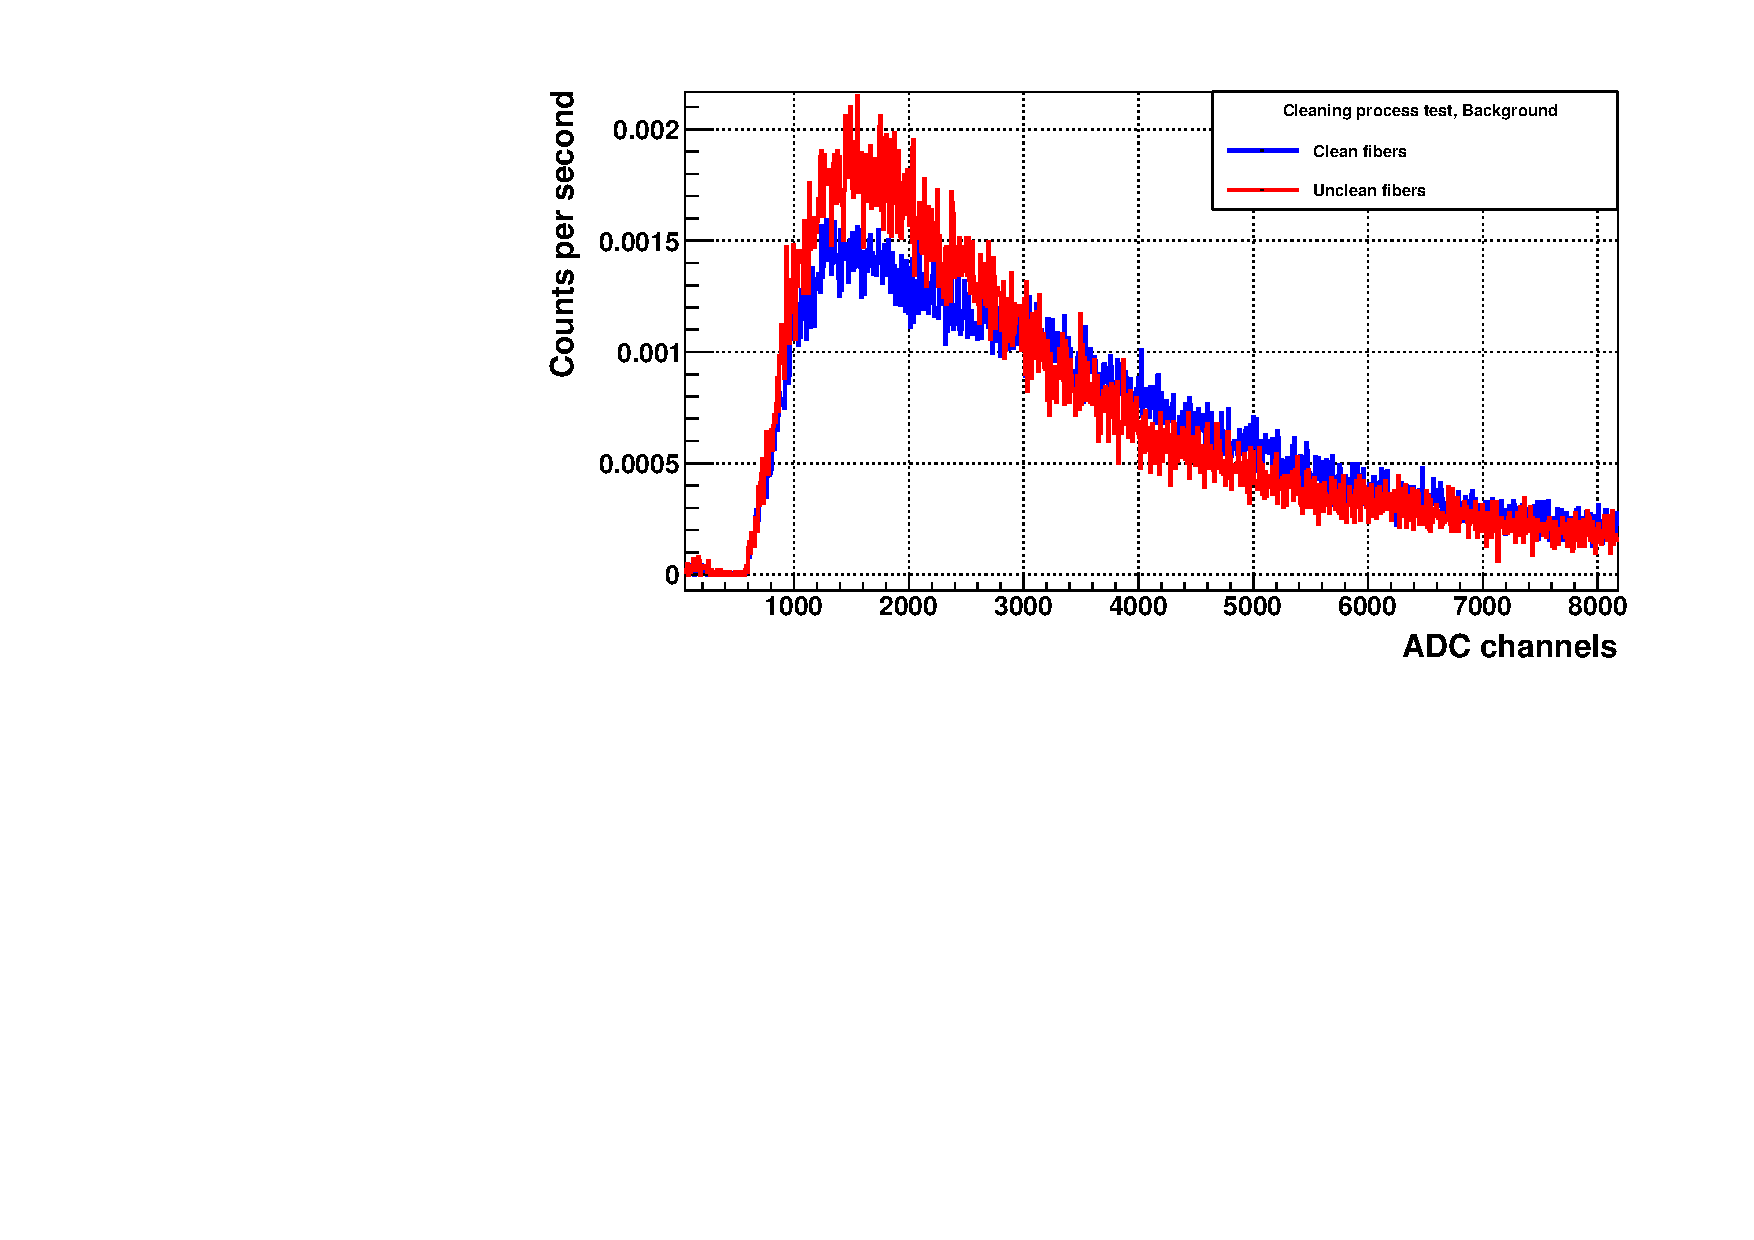
\includegraphics[scale=0.6]{4ResearchAndDevelopments/41Fibers/Background_CleaningProcess.pdf}
\caption{Measured background energy spectra before and after cleaning.\label{fig:ResultsOfCleaningProcessBackground}}
\end{figure}

\begin{figure}
\centering
    \begin{subfigure}[b]{1\textwidth}
    \centering
    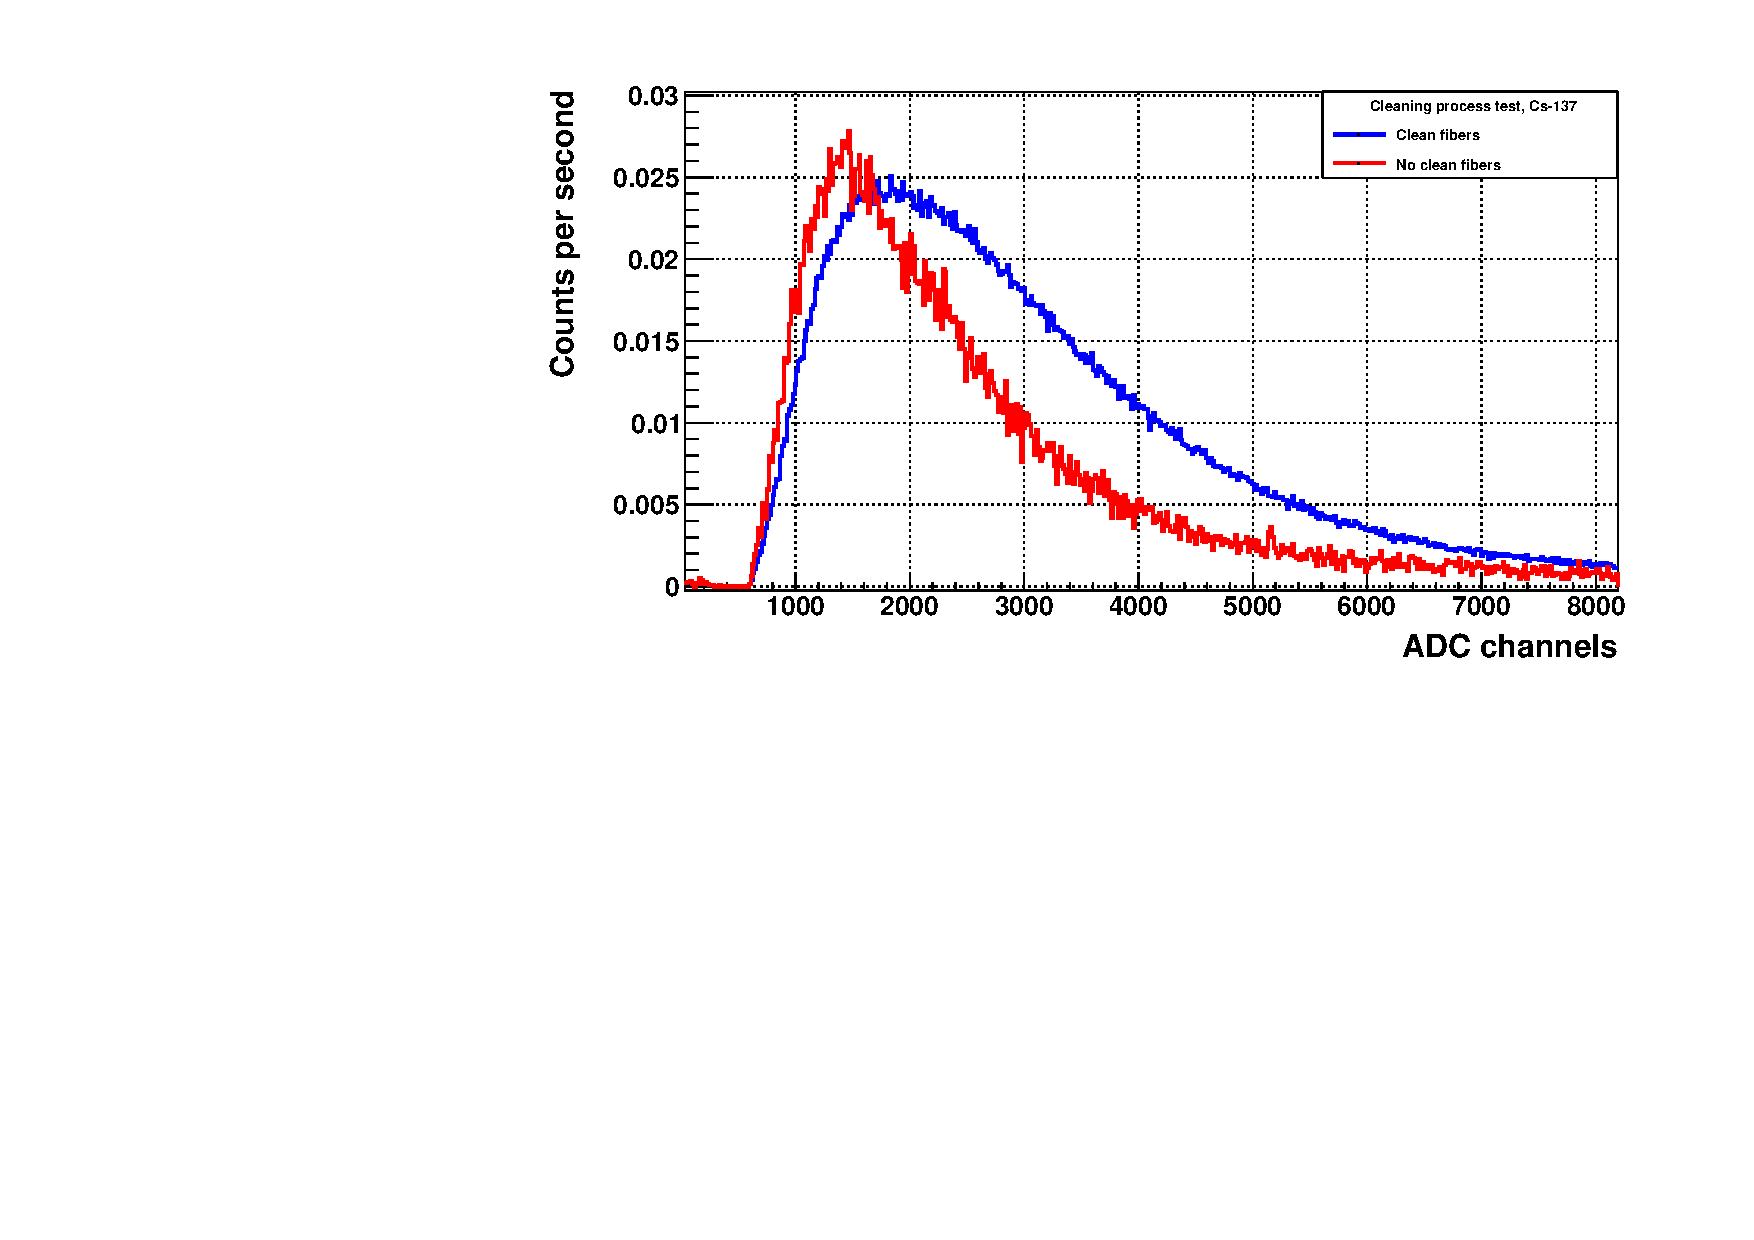
\includegraphics[width=\textwidth]{4ResearchAndDevelopments/41Fibers/Cs-137_CleaningProcess.pdf}  
    \caption{\label{subfig:EnergySpectrumCo60CleaningTest}}
    \end{subfigure}
    \hfill
    \begin{subfigure}[b]{1\textwidth}
    \centering
    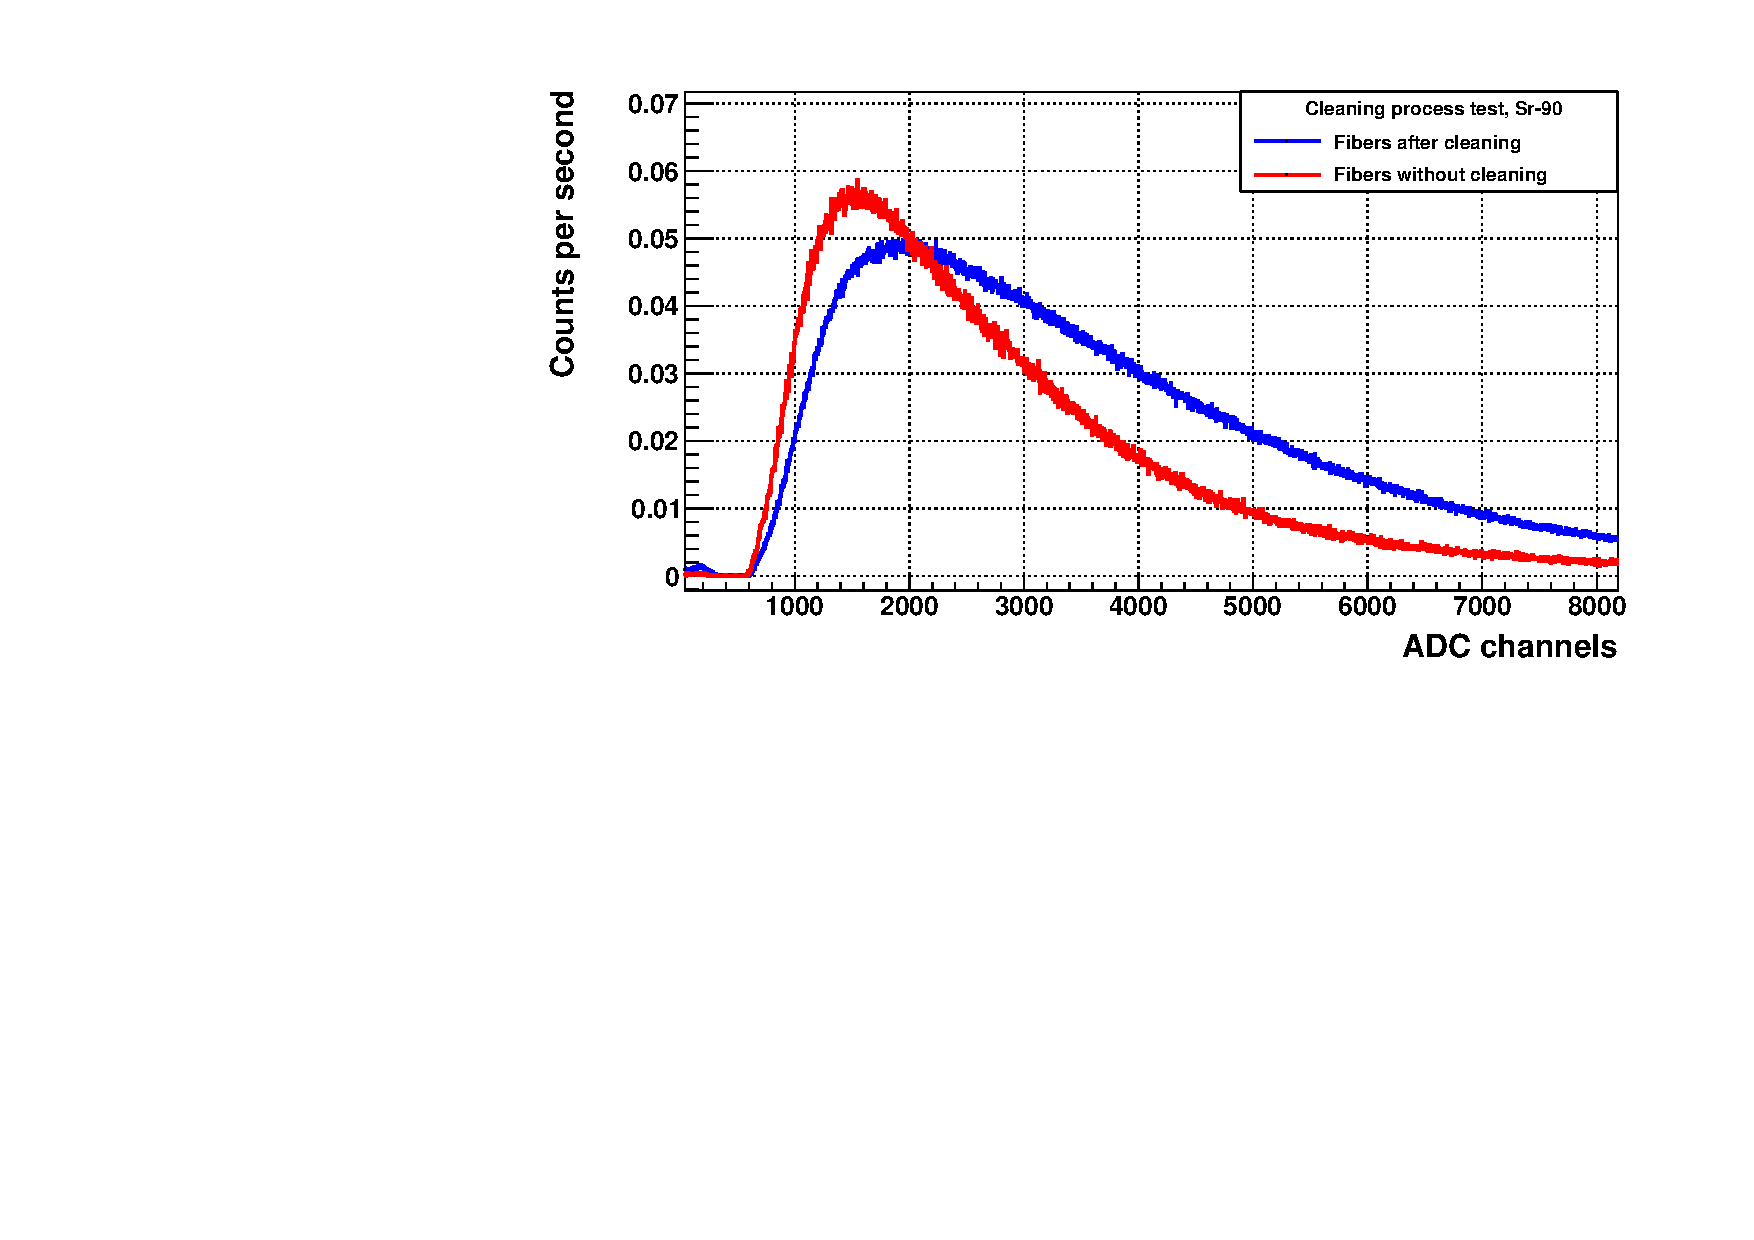
\includegraphics[width=\textwidth]{4ResearchAndDevelopments/41Fibers/Sr-90_CleaningProcess.pdf}  
    \caption{\label{subfig:EnergySpectrumSr90CleaningTest}}
    \end{subfigure}
 \caption{Energy spectra obtained before and after the cleaning for a radioactive source. a) $\ce{^{137}Cs}$. b) $\ce{^{90}Sr}$.}
 \label{fig:ResultsOfCleaningProcessSource}
\end{figure}


%$(27.73 \pm 1.6)\%$ for the gamma source and $(20.72 \pm 0.9)\%$ for the beta source so, the improvement of the photon collection efficiency of the fibres was verified using the cleaning process carried out in the clean room of ICMOL laboratories. Nevertheless, it should be taken into accout that this test was carried out in air. It could be interesting to repeat it in water to obtain more realistic conclusions since the fibres of the TRITIUM detector will be immersed in water.